\chapter{الموجات، والأنماط المكمّاة، ومؤثرات الخلق}

\section{الموجات، والحقول، والأسّيات المركبة}

نظرية الحقل الكمومي هي الأداة الأساسية لفيزياء الجسيمات. وقبل تقديم حتى عرض أولي لحقل كمومي، من المفيد جمع الحقائق الرياضية التي تصل بين الموجات والجسيمات. فالموجة هي بالفعل تهيئة حقلية: إذ يتغيّر الحقل من نقطة إلى أخرى في الفضاء، والموجة تهيئة تتذبذب فيها تلك القيم وتنتشر. وتوفّر ميكانيكا الكم الصلة بين مثل هذه الموجات والجسيمات.

يُفترض هنا الإلمام المسبق بميكانيكا الكم والنسبية الخاصة. والغرض المباشر هو مراجعة العناصر اللازمة لفيزياء الجسيمات، لا أن يحل هذا محل مقرر في أيٍّ من الموضوعين.

تتميّز الدالة الأسية بنمو متناسب. فإذا
\begin{equation}
f(x)=e^{\alpha x},
\end{equation}
فحينئذٍ
\begin{equation}
\frac{df}{dx}=\alpha f.
\end{equation}
فعلى مدى فترة صغيرة، تكون الزيادة متناسبة مع المقدار الموجود سلفًا. ويعطي نمو جماعة من الكائنات في طبق بتري الصورة المألوفة: فكلما ازداد عدد الكائنات الموجودة، ازداد ما هو متاح منها للتكاثر، لذا يكون معدل الازدياد متناسبًا مع الجماعة نفسها. ولا يغيّر ضرب \(e^{\alpha x}\) في ثابت كلي هذه الخاصية التعريفية.

تتذبذب دالتا الجيب وجيب التمام بدلًا من النمو. وهما المنحنى نفسه مزاحًا بمقدار ربع دورة، والاشتقاق يحوّل كلًّا منهما إلى الآخر:
\begin{align}
\frac{d}{dx}\sin(kx)&=k\cos(kx),\\
\frac{d}{dx}\cos(kx)&=-k\sin(kx).
\end{align}
وليست أيٌّ من الدالتين وحدها دالةً أسية، لأن مشتقتها تتناسب مع الدالة الأخرى. أما التركيب المركب فله الخاصية الأسية فعلًا. ومع \(i^2=-1\)،
\begin{align}
\frac{d}{dx}\bigl(\cos(kx)+i\sin(kx)\bigr)
&=-k\sin(kx)+ik\cos(kx)\\
&=ik\bigl(\cos(kx)+i\sin(kx)\bigr).
\end{align}
ولذلك
\begin{equation}
e^{ikx}=\cos(kx)+i\sin(kx).
\end{equation}
وتظهر هذه المتطابقة مرارًا لأن الجيب وجيب التمام يصفان تذبذبات شبيهة بالموجات. فعندما يكون \(x\) إحداثيًا مكانيًا، تتذبذب الدالة عبر الفضاء. وعندما تكون الحجة زمنًا، فإنها تتذبذب في الزمن.

\section{التردد، والطول الموجي، وزخم الفوتون}

التردد المعتاد \(f\) هو عدد الدورات الكاملة في الثانية. وتعني الدورة اهتزازة كاملة واحدة. ويقيس التردد الزاوي الحركة نفسها بوحدة الراديان في الثانية:
\begin{equation}
\omega=2\pi f.
\end{equation}
والترميزان يصفان التردد نفسه. وينتقل المرء بينهما لإبقاء عوامل \(2\pi\) غير الضرورية خارج الحساب، مع أن هذه العوامل لا تختفي تمامًا أبدًا.

الطول الموجي \(\lambda\) هو المسافة التي تشغلها دورة مكانية كاملة واحدة. فإذا انتشرت موجة بسرعة \(v\)، فإن المسافة في كل دورة مضروبة في عدد الدورات في الثانية هي سرعة الانتشار:
\begin{equation}
\lambda f=v.
\end{equation}
وبالنسبة إلى الضوء في الفراغ، \(v=c\)، ولذلك
\begin{equation}
\lambda f=c.
\end{equation}
أما في موجة صوتية فالطرف الأيمن هو سرعة الصوت، وفي موجة مائية هو سرعة الموجة المائية المناسبة. ومن ثم فإن ظهور \(c\) هو قول عن الضوء، لا تعريفًا مشتركًا لكل موجة.

تقدّم ميكانيكا الكم ثابت بلانك بترميزين،
\begin{equation}
\hbar=\frac{h}{2\pi}.
\end{equation}
والانتقال من \(h\) إلى \(\hbar\) لا يفعل إلا نقل عوامل \(2\pi\) من معادلة إلى أخرى.

تعتمد القيم العددية للثوابت ذات الأبعاد على الوحدات المستخدمة للتعبير عنها. فالمتر والثانية والكيلوغرام اصطلاحات على المقياس البشري، ملائمة للأطوال والأزمنة العادية. وكانت الوحدات التقليدية القريبة من طول الذراع مفيدة للقماش أو الحبال؛ ومهما يكن المسار التاريخي الدقيق الذي أدى إلى المتر، فلا يوجد مبدأ أساسي يختار هذا المقياس البشري بعينه. وفي وحدات النظام الدولي SI،
\begin{equation}
\begin{aligned}
h &\simeq 6.6\times10^{-34}\ \mathrm{J\,s},
&\hbar &\simeq 1.1\times10^{-34}\ \mathrm{J\,s},\\
c &\simeq 3\times10^8\ \mathrm{m\,s^{-1}}.
\end{aligned}
\end{equation}
والمغزى من هذه الأرقام هو مقياسها في الوحدات الاصطلاحية: فثابت بلانك صغير على نحو غير عادي، وسرعة الضوء كبيرة على نحو غير عادي.

لكمّ واحد من نمط طاقة
\begin{equation}
E_{\text{one quantum}}=\hbar\omega=hf.
\end{equation}
وهذه هي طاقة فوتون واحد، لا الطاقة الكلية لموجة كهرومغناطيسية كلاسيكية اعتباطية. فللضوء المرئي تردد من رتبة \(10^{15}\) دورة في الثانية، ولذلك تكون طاقة فوتون ضوئي نموذجي من رتبة
\begin{equation}
E_\gamma\sim 10^{-19}\ \mathrm{J}.
\end{equation}
وحتى مثل هذا التذبذب البصري السريع يعطي طاقة صغيرة جدًا لكل كم لأن \(h\) صغير جدًا. ولذلك فإن مقدارًا ماكروسكوبيًا من الطاقة الضوئية يحتوي على عدد هائل من الفوتونات.

تستحق الطاقة والزخم عناية خاصة لأن كليهما محفوظ. وهما كميتان مفيدتان لضبط الحساب: إذ يجب أن تتوازن الطاقة والزخم الكليان الداخلان في عملية ما مع الطاقة والزخم الكليين الخارجين منها. والزخم متجه ويشير في اتجاه الحركة. وبالنسبة إلى جسيم يتحرك أبطأ كثيرًا من الضوء،
\begin{equation}
\vec p=m\vec v.
\end{equation}

والآن انظر في إشعاع كهرومغناطيسي مُحزَّم على امتداد اتجاه واحد، بدلًا من أن يكون مبعثرًا في اتجاهات كثيرة. ويتجه زخمه على طول الحزمة. ولا يمكن تطبيق الصيغة غير النسبية على الفوتون، لأن \(m\) تعني كتلة السكون، وكتلة سكون الفوتون صفر. ومع ذلك توجد وسيلة تذكّر بُعدية مفيدة. فإذا أسند المرء إلى الفوتون، \emph{على نحو غير ملائم}، الكمية \(E/c^2\) كما لو كانت كتلةً ثم عوّض \(v=c\)، وجد
\begin{equation}
mv\longrightarrow \frac{E}{c^2}c=\frac{E}{c}.
\end{equation}
وتصادف أن هذه الحيلة تعطي الجواب الصحيح وتجعل الوحدات صحيحة، لكنها ليست حجة مشروعة على أن للفوتون كتلة سكون \(E/c^2\). أما العبارة النسبية الصحيحة للإشعاع المُحزَّم فهي
\begin{equation}
|\vec p|=\frac{E}{c}.
\end{equation}
وتعطي المعادلة المقدار. أما الاتجاه فهو الاتجاه الذي يسير فيه الإشعاع.

بالنسبة إلى فوتون واحد،
\begin{align}
|\vec p_\gamma|
&=\frac{E_\gamma}{c}
=\frac{hf}{c}.
\end{align}
وبالنسبة إلى الضوء،
\begin{equation}
\lambda f=c,
\qquad
\frac{f}{c}=\frac{1}{\lambda},
\end{equation}
ومن ثم
\begin{equation}
|\vec p_\gamma|=\frac{hf}{c}=\frac{h}{\lambda}.
\end{equation}

\begin{figure}[t]
\centering
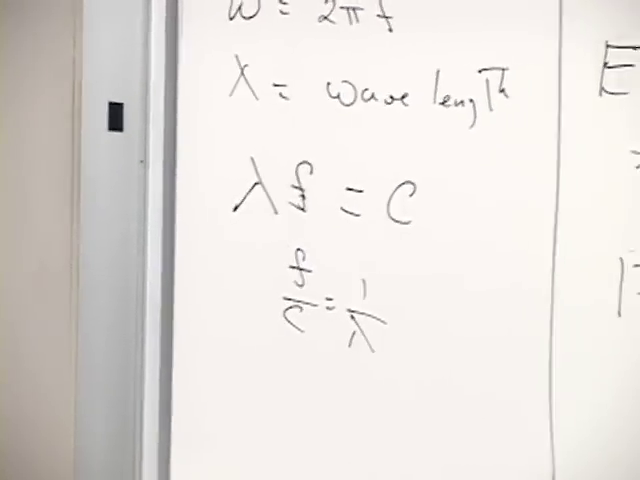
\includegraphics[width=0.56\textwidth]{lecture_02_figure_02.png}
\caption{بالنسبة إلى الضوء، \(\lambda f=c\) و\(f/c=1/\lambda\) هما العلاقتان المستخدمتان لاستخراج \(|\vec p_\gamma|=h/\lambda\).}
\lectureframe{00:21:39}
\end{figure}

كلما قصر الطول الموجي، ازداد زخم الفوتون. وهذه إحدى أهم الحقائق الكمومية في فيزياء الجسيمات. فلدراسة جسم صغير يحتاج المرء إلى مسبار قصير الطول الموجي، وثمن ذلك القِصر في الطول الموجي هو زخم كبير.

\begin{classroomqa}
\lecturetimestamp{00:22:23}
\audiencequestion{هل \(E=\hbar\omega\) أساسي، أم إنه مشتق من مبدأ أعمق؟}
\lecturerresponse{ينتج ذلك من ميكانيكا الكم للمذبذب التوافقي. وستُستخدم هذه النتيجة هنا من دون إعادة برهانها؛ وتوفّر لغة المذبذب التي ستُطوَّر أدناه الإطار الأعمق لها.}
\end{classroomqa}


\section{سعة الموجة وعدد الفوتونات}

\begin{classroomqa}
\lecturetimestamp{00:23:10}
\audiencequestion{ماذا تعني سعة الموجة بلغة الفوتونات؟}
\lecturerresponse{قارن بين موجتين لهما الطول الموجي والتردد نفسيهما ولكن بسعتين مختلفتين، مثل \(\sin(kx)\) و\(A\sin(kx)\). وكلاسيكيًا، تكون الطاقة في منطقة ثابتة متناسبة مع مربع السعة. وكموميًا، يكون للنمط الذي يحتوي على \(n\) فوتونًا طاقة \(n\hbar\omega\). ولذلك، عند تثبيت التردد والمنطقة والتطبيع، تنمو السعة، من حيث رتبة المقدار، مثل \(\sqrt n\).}
\end{classroomqa}

الموجتان متماثلتان في نمط تذبذبهما. وإحداهما ببساطة أشد من الأخرى.\footnote{يوضّح الرسم التخطيطي مقارنة الموجتين عند 00:23:47--00:24:28.}

\begin{figure}[t]
\centering
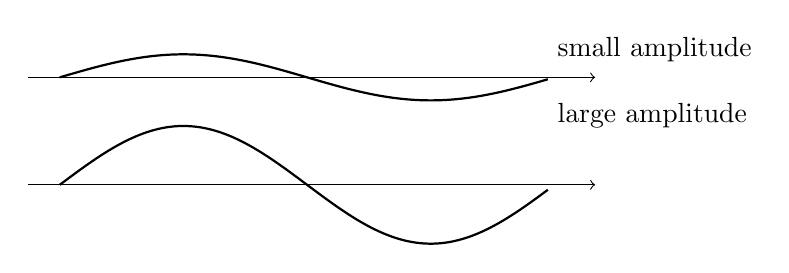
\begin{tikzpicture}[x=1cm,y=0.65cm]
\draw[->] (-0.4,0) -- (6.8,0);
\draw[->] (-0.4,-2.1) -- (6.8,-2.1);
\draw[thick] plot[domain=0:6.2,samples=120] (\x,{0.45*sin(\x r)});
\draw[thick] plot[domain=0:6.2,samples=120] (\x,{-2.1+1.15*sin(\x r)});
\draw (6.2,0.55) node[right]{small amplitude};
\draw (6.2,-0.75) node[right]{large amplitude};
\end{tikzpicture}
\caption{موجات لها الطول الموجي والتردد نفسيهما ولكن بسعات مختلفة.}
\end{figure}

لمقدار ثابت من الموجة،
\begin{equation}
E_{\text{wave}}\propto A^2.
\end{equation}
وبالنسبة إلى موجة كهرومغناطيسية، فهذا هو القول المألوف إن طاقة الحقل تتناسب مع مربع شدة الحقل. وإذا احتوى النمط نفسه على \(n\) فوتونًا، فإن
\begin{equation}
E_{\text{wave}}=n\hbar\omega.
\end{equation}
وبالتالي، مع تثبيت النمط والتردد والتطبيع والمنطقة،
\begin{equation}
A^2\propto n\hbar\omega,
\qquad
A\propto\sqrt n\quad\text{at fixed }\omega.
\end{equation}
ولا يُدَّعى هنا أي تطبيع دقيق. فمقدار الموجة المشمول مهم: إذ إن مضاعفة طول موجة منتظمة فيما عدا ذلك تغيّر طاقتها الكلية من دون أن تغيّر السعة الموضعية. ولذلك يمكن فهم التناسب على أنه يخص منطقة ثابتة، مثل طول موجي واحد.

وهناك أيضًا تحفّظ كمّي مخصوص. فلا يمكن إسناد قيم كلاسيكية مضبوطة تمامًا إلى السعة والطور معًا. ولذلك يكون السؤال ``ما سعة فوتون واحد؟'' ملتبسًا إذا كان يطلب حقلًا كلاسيكيًا محددًا على نحو حاد تمامًا. ومع ذلك، فإن اتخاذ \(n=1\) يعطي مقياسًا معقولًا لرتبة المقدار.

\begin{classroomqa}
\lecturetimestamp{00:28:25}
\audiencequestion{هل تمثّل الإزاحة العمودية في رسم موجة كهرومغناطيسية موضع الفوتون في الفضاء؟}
\lecturerresponse{لا. فمحور الانتشار مكاني، في حين يمثّل الإحداثي العمودي قيمة المجال الكهربائي أو المغناطيسي. ويتجه الزخم على طول محور الانتشار، لا على طول سعة الحقل المرسومة.}
\end{classroomqa}

قد تنتشر الموجة في أي اتجاه مكاني، لكن الرسم الجيبي المألوف يستخدم محوره الأفقي وحده بوصفه إحداثيًا مكانيًا. أما الاتجاه الآخر المرسوم فيسجّل شدة الحقل.

\begin{classroomqa}
\lecturetimestamp{00:29:37}
\audiencequestion{هل يُعَدّ عدد الفوتونات المذكور داخل طول موجي واحد أم داخل دورة واحدة من الموجة؟}
\lecturerresponse{يمكن اختيار منطقة ثابتة، مثل طول موجي واحد. ولهذا فالعلاقة تناسبية فحسب: إذ تعتمد الطاقة الكلية وعدد الفوتونات أيضًا على مقدار ما يُضمَّن من الموجة. فطولان موجيان أو ثلاثة أو أربعة أطوال موجية تحتوي، عند السعة نفسها، على طاقة أكبر تبعًا لذلك من طول موجي واحد.}
\end{classroomqa}

\begin{classroomqa}
\lecturetimestamp{00:30:17}
\audiencequestion{هل سعة فوتون واحد بلا معنى؟}
\lecturerresponse{لا تكون ذات معنى إلا بوصفها عبارة عن رتبة مقدار تُستحصل بوضع \(n=1\). بالنسبة إلى نمط كهرومغناطيسي، تؤدي معلومات المجالين الكهربائي والمغناطيسي دورًا مماثلًا لمعلومات الموضع والزخم المترافقين، لذا يحد عدم اليقين الكمومي من مدى إمكان تعيين سعة كلاسيكية تعيينًا حادًا. وتظل علاقة رتبة المقدار مفيدة.}
\end{classroomqa}

تقود هذه الأسئلة بالفعل إلى نظرية الحقل الكمومي، حيث يمكن بيان العلاقة بين متغيرات الحقل وعدد الجسيمات على نحو دقيق. أما الآن فتكفي علاقات التناسب.

\section{العلاقات الكمومية العامة وموجات المادة البطيئة}

تنطبق بعض الصيغ التي قُدِّمت للفوتونات على نحو أعم بكثير، بينما لا تنطبق صيغ أخرى كذلك. ومن المفيد فرزها قبل الانتقال إلى الإلكترونات.

\begin{figure}[t]
\centering
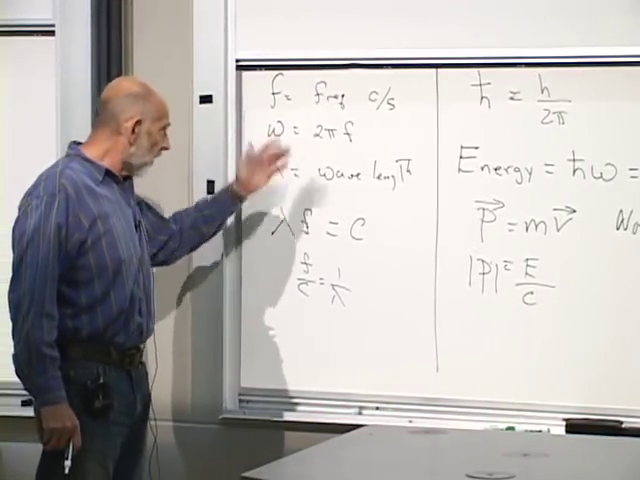
\includegraphics[width=0.82\textwidth]{lecture_02_figure_03.png}
\caption{تعريفات الموجات، وعلاقتا الزخم للفوتون وللحركة غير النسبية، مقارنةً بحسب مجالات صلاحيتهما.}
\lectureframe{00:31:52}
\end{figure}

تنطبق تعريفات \(f\) و\(\omega=2\pi f\) و\(\lambda\) على نحو عام. كما أن العلاقة الكمومية
\begin{equation}
E=\hbar\omega=hf
\end{equation}
عامة أيضًا في المناقشة الحالية. وعلى النقيض من ذلك، فإن الصيغ التي تتضمن \(c\)، مثل \(\lambda f=c\) و\(|\vec p|=E/c\)، تنطبق على الموجات التي تتحرك بسرعة الضوء. أما الصيغة \(\vec p=m\vec v\) فتنطبق على الجسيمات التي تتحرك أبطأ بكثير من الضوء. وتتطلب الحركة النسبية بين هذين الحدين استيفاءً ليس مطلوبًا بعد.

لا تقتصر علاقة الزخم--الطول الموجي على مثال الفوتون:
\begin{equation}
p=\frac{h}{\lambda}.
\end{equation}
وهنا يدل \(p\) على المقدار عندما تُؤخذ \(\lambda\) بوصفها طولًا موجيًا موجبًا؛ ويمكن تحديد الاتجاه على نحو منفصل.

\begin{figure}[t]
\centering
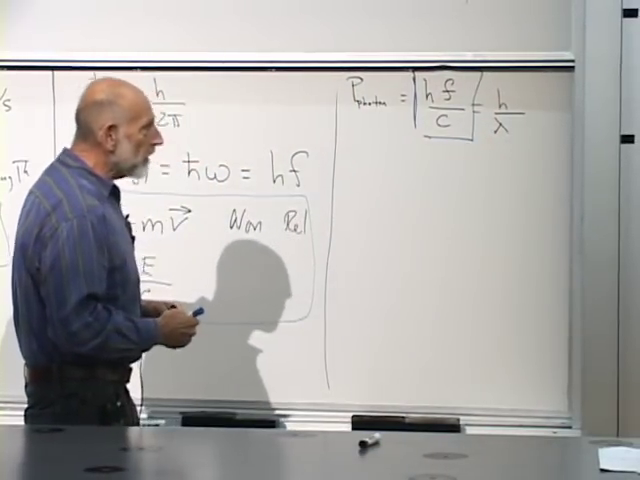
\includegraphics[width=0.74\textwidth]{lecture_02_figure_04.png}
\caption{زخم الفوتون \(|\vec p_\gamma|=hf/c=h/\lambda\)، مما يقود إلى علاقة دي برولي العامة.}
\lectureframe{00:33:32}
\end{figure}

يمكن ربط إلكترون، ونواة، وحتى كرة بولينغ، بموجة. ويُعد تداخل الإلكترونات أحد تجليات هذه الحقيقة. اكتب موجة الإلكترون على الصورة \(\psi\). ما الذي يحل محل \(\lambda f=c\) لإلكترون يتحرك ببطء؟ العنصر الناقص هو العلاقة غير النسبية بين الطاقة والزخم.

نبدأ بالطاقة الحركية والزخم:
\begin{align}
E&=\frac12 mv^2,\\
p&=mv,
\qquad
v=\frac{p}{m}.
\end{align}
وبالتعويض من العلاقة الأخيرة في الأولى نحصل على
\begin{align}
E
&=\frac12m\left(\frac{p}{m}\right)^2\\
&=\frac{p^2}{2m}.
\end{align}
تظهر الكتلة في البسط في \(\frac12 mv^2\) وفي المقام في \(p^2/(2m)\). ومن السهل الالتباس في هذا الترتيب، ومن المفيد إعادة اشتقاقه.

والآن نستخدم العلاقات الكمومية العامة
\begin{equation}
E=hf,
\qquad
p=\frac{h}{\lambda}.
\end{equation}
وبالنسبة إلى جسيم بطيء واحد،
\begin{align}
hf
&=\frac{p^2}{2m}\\
&=\frac{1}{2m}\left(\frac{h}{\lambda}\right)^2\\
&=\frac{h^2}{2m\lambda^2}.
\end{align}
وبالقسمة على \(h\) نحصل على
\begin{equation}
f=\frac{h}{2m\lambda^2}.
\end{equation}

\begin{figure}[t]
\centering
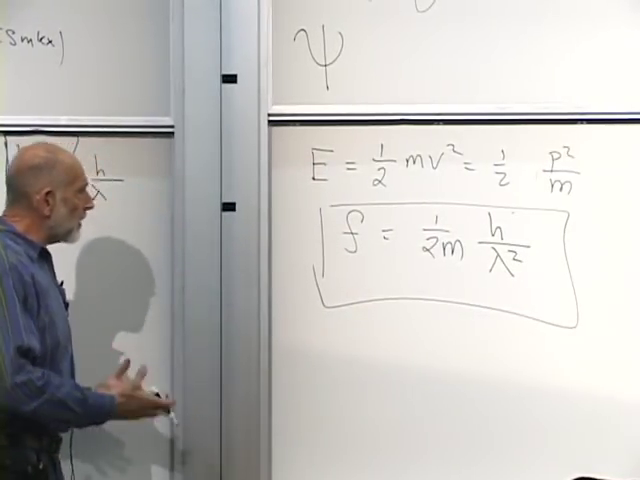
\includegraphics[width=0.64\textwidth]{lecture_02_figure_05.png}
\caption{بالنسبة إلى جسيم بطيء، تؤدي \(E=p^2/(2m)\) و\(p=h/\lambda\) إلى \(f=h/(2m\lambda^2)\).}
\lectureframe{00:37:47}
\end{figure}

بالنسبة إلى الضوء،
\begin{equation}
f\propto\frac{1}{\lambda},
\end{equation}
أما بالنسبة إلى المادة البطيئة،
\begin{equation}
f\propto\frac{1}{\lambda^2}.
\end{equation}
فلا حاجة إلى حفظ العلاقة الثانية بمعزل عن غيرها. إذ يمكن دائمًا إعادة بنائها انطلاقًا من \(E=p^2/(2m)\) و\(E=hf\) و\(p=h/\lambda\). وبالنسبة إلى إلكترون يتحرك ببطء في ذرة، فإنها تعطي تردد موجة Schr\"odinger الموافقة.

\begin{classroomqa}
\lecturetimestamp{00:38:35}
\audiencequestion{هل تنطبق علاقة التردد--الطول الموجي غير النسبية على جسيمات أخرى غير الإلكترونات؟}
\lecturerresponse{نعم. إنها تنطبق على أي جسيم يتحرك أبطأ بكثير من الضوء. أما الاستيفاء النسبي بين الحد البطيء والحد الضوئي فهو موضوع مستقل.}
\end{classroomqa}

\begin{classroomqa}
\lecturetimestamp{00:38:55}
\audiencequestion{ما العلاقة التي تنطبق على نيوترينو؟}
\lecturerresponse{يعتمد ذلك على سرعة النيوترينو. فمعظم النيوترينوهات التي نصادفها في الطبيعة تتحرك بسرعة قريبة جدًا من سرعة الضوء، لذا تكون علاقة الحد الضوئي تقريبًا جيدًا. أما النيوترينو الذي يتحرك أبطأ بكثير من الضوء فيخضع بدلًا من ذلك للعلاقة غير النسبية.}
\end{classroomqa}

\editorialnote{يتناول تبادل قصير مع الحضور، مباشرة بعد سؤال النيوترينو، السعات والكمّات واختلاف الأطوال الموجية للإلكترونات، لكن صياغته متضررة أكثر مما يسمح باستعادتها على نحو موثوق. أما الرد الذي أمكن استخلاصه فيؤجل العلاقة العامة بين السعات والكمّات ذات الأطوال الموجية المختلفة.}

\begin{classroomqa}
\lecturetimestamp{00:39:56}
\audiencequestion{هل يكون إلكترون من مسرّع \(20\,\mathrm{keV}\) بطيئًا أم نسبيًا؟}
\lecturerresponse{يُعامل على أنه بطيء. ففي الوحدات التي يكون فيها \(c=1\)، يمكن التعبير عن الكتلة والطاقة والزخم بالوحدات نفسها. ويبلغ مقياس طاقة السكون للإلكترون تقريبًا \(0.5\,\mathrm{MeV}\)، في حين أن \(20\,\mathrm{keV}\) أصغر بكثير. وبصورة مكافئة، فإن معيار الزخم غير النسبي هو \(p\ll mc\).}
\end{classroomqa}

مقارنة الطاقة في المثال هي
\begin{equation}
K=20\,\mathrm{keV}\ll m_ec^2\simeq0.5\,\mathrm{MeV}.
\end{equation}
\editorialnote{يعرض المقطع الأصلي عند 00:39:56--00:41:40 القيمة \(20\,\mathrm{keV}\) بوصفها طاقة مسرّع، ثم يصوغ المعيار النسبي بدلالة مقارنة الزخم بكتلة السكون. إن كتابة معياري الطاقة الحركية والزخم كلٌّ على حدة تتجنب مساواة الطاقة المذكورة بزخم، مع الحفاظ على الاستنتاج غير النسبي المذكور.}

\section{سرعة الطور، وسرعة المجموعة، والتشتت}

\begin{classroomqa}
\lecturetimestamp{00:41:46}
\audiencequestion{هل يمكن استخدام حاصل ضرب التردد في الطول الموجي للحصول على سرعة موجة إلكترون؟}
\lecturerresponse{إنه يعطي سرعة الطور، لا السرعة المنسوبة إلى الإلكترون. وللحزمة الموضعية كلٌّ من سرعة طور تصف حركة قممها وقيعانها الداخلية، وسرعة مجموعة تصف حركة الغلاف. وتُعرَّف سرعة المجموعة بأنها السرعة الموافقة لحركة الجسيم.}
\end{classroomqa}

تبدو الحزمة الموجية محليًا كموجة جيب أو جيب تمام، لكنها محصورة بغلاف. وأثناء حركتها، لا يلزم أن يتحرك الغلاف والقمم الموجودة داخله بالسرعة نفسها.\footnote{يتبع هذا الرسم التخطيطي مناقشة الحزمة الموجية عند 00:42:34--00:44:11.}

\begin{figure}[t]
\centering
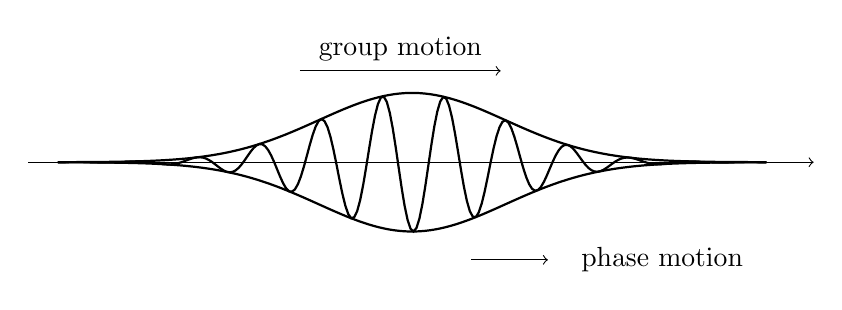
\begin{tikzpicture}[x=0.75cm,y=0.8cm]
\draw[->] (-0.5,0) -- (12.8,0);
\draw[thick] plot[domain=0:12,samples=140] (\x,{1.10*exp(-0.20*(\x-6)^2)});
\draw[thick] plot[domain=0:12,samples=140] (\x,{-1.10*exp(-0.20*(\x-6)^2)});
\draw[thick] plot[domain=0:12,samples=240] (\x,{1.10*exp(-0.20*(\x-6)^2)*sin(6*\x r)});
\draw[->] (4.1,1.45) -- (7.5,1.45);
\draw (5.8,1.8) node{group motion};
\draw[->] (7.0,-1.55) -- (8.3,-1.55);
\draw (8.7,-1.55) node[right]{phase motion};
\end{tikzpicture}
\caption{حزمة موجية موضعية يتحرك غلافها وطورها الداخلي عمومًا بسرعات مختلفة.}
\end{figure}

سرعة الطور هي سرعة القمم والقيعان وسائر الأطوار الثابتة لمركبة وحيدة التردد. وبالنسبة إلى علاقة التشتت غير النسبية،
\begin{equation}
v_\phi=f\lambda=\frac{h}{2m\lambda}.
\end{equation}
فهي تعتمد على الطول الموجي. ولذلك تكون لمركبات الأطوال الموجية المختلفة سرعات طور مختلفة، ومن ثم يمكن للقمم أن تتحرك عبر الحزمة ويمكن للحزمة أن تتشتت. أما سرعة المجموعة فهي سرعة الحزمة ككل، وهي التي تُعرَّف بوصفها سرعة الجسيم.

توجد حالة خاصة بسيطة. فإذا تحركت جميع مركبات الأطوال الموجية بالسرعة نفسها، اتفقت سرعتا الطور والمجموعة. وللضوء في الفراغ هذه الخاصية: فكل طول موجي ينتشر بسرعة \(c\). أما علاقة الجسيم البطيء فلا تملكها؛ إذ إن \(f\lambda\) فيها يتغير مع \(\lambda\).

المعادلة
\begin{equation}
f=\frac{h}{2m\lambda^2}
\end{equation}
هي معادلة Schr\"odinger الحرة في صورة مموهة قليلًا. يحدد التردد الاعتماد الزمني لموجة مستوية، ويحدد الطول الموجي اعتمادها المكاني، وتربط معادلة Schr\"odinger بينهما. وعلى العكس، فإن إدخال موجة ذات تردد معيّن وطول موجي معيّن في معادلة Schr\"odinger الحرة يعيد إنتاج علاقة التشتت هذه.

\begin{classroomqa}
\lecturetimestamp{00:47:02}
\audiencequestion{هل يمكن أن تتجاوز سرعة الطور سرعة الضوء؟}
\lecturerresponse{نعم. سرعة الطور لا تنقل معلومات. أما المعلومات والحزمة الموضعية فتنتشران بسرعة المجموعة، لذا لا تتيح سرعة طور فوق ضوئية إرسال إشارات فوق ضوئية.}
\end{classroomqa}

\section{الفضاء المحدود والزخم المتقطع}

الغاية النهائية هي الموجات في فضاء لانهائي، لكن البدء بنظام محدود أكثر أمانًا. فاللانهاية ليست شيئًا يستطيع الحاسوب تخزينه أو معالجته مباشرة. تُصاغ المعادلات أولًا لنظام محدود، ثم لا يُؤخذ إلا بعد ذلك الحد الذي يصبح فيه حجمه كبيرًا كيفما نشاء. وهذه العادة مفيدة في ميكانيكا الكم، ونظرية الحقل الكمومي، وفيزياء الجسيمات كلها.

لا يضيع شيء أساسي بالبدء في بعد مكاني واحد. فقد تعيش الموجة على وتر كمان، أو على حبل يُهز، أو في عالم تجريدي أحادي البعد. وأوضح نظام محدود هو قطعة طولها \(L\) ذات طرفين عاكسين. تنتقل موجة إلى أحد الطرفين، فتنعكس، ثم تعود. هذا شرط حدود عاكس مشروع تمامًا، لكنه ينطوي على إزعاج: فالزخم غير محفوظ داخل النظام الموجي. فالموجة المتحركة نحو اليمين تحمل زخمًا يمينيًا؛ وبعد الانعكاس تحمل زخمًا يساريًا. وقد وفّر الحدّ الدفعة وامتص الفرق.

يمكن تمثيل انقلاب الزخم عند طرف عاكس تمثيلًا تخطيطيًا.\footnote{يتبع هذا الرسم التخطيطي الحجة المتعلقة بالحدود العاكسة عند 00:49:24--00:51:08.}

\begin{figure}[t]
\centering
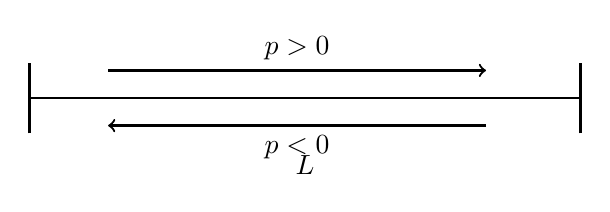
\begin{tikzpicture}[x=1cm,y=1cm]
\draw[thick] (0,0) -- (7,0);
\draw[very thick] (0,-0.45) -- (0,0.45);
\draw[very thick] (7,-0.45) -- (7,0.45);
\draw[->,thick] (1.0,0.35) -- (5.8,0.35) node[midway,above]{\(p>0\)};
\draw[->,thick] (5.8,-0.35) -- (1.0,-0.35) node[midway,below]{\(p<0\)};
\draw (3.5,-0.85) node{\(L\)};
\end{tikzpicture}
\caption{الانعكاس عند طرفي قطعة محدودة يقلب اتجاه زخم موجة منتقلة.}
\end{figure}

هناك طريقة أخرى لجعل النظام منتهيًا مع الحفاظ على الزخم. اجعل طرفي القطعة متطابقين. يمكن رسم النتيجة على هيئة دائرة، لكن لا حاجة إلى دائرة حرفية مضمَّنة في بُعد ثانٍ. والصياغة الرياضية هي ببساطة أن الإحداثي دوري: فبعد قطع مسافة كلية مقدارها \(L\) يعود المرء إلى النقطة نفسها.

\begin{figure}[t]
\centering
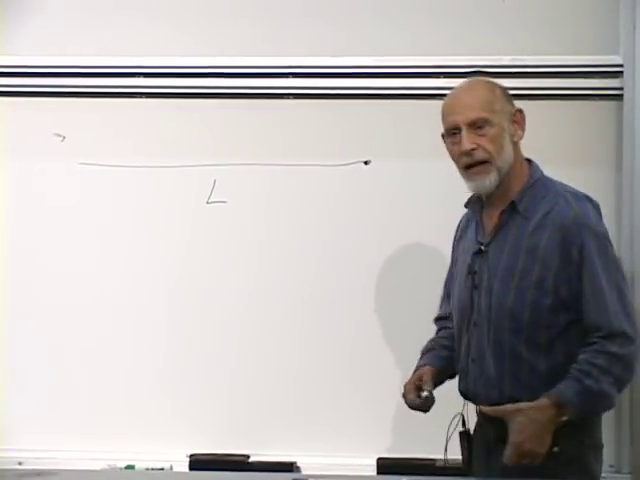
\includegraphics[width=0.72\textwidth]{lecture_02_figure_06.png}
\caption{مسار أحادي البعد بطول كلي \(L\) يُستخدم لتقديم المطابقة الدورية.}
\lectureframe{00:51:21}
\end{figure}

يُصرَّح بتطابق الطرفين في المخطط الآتي.\footnote{ويتبع هذا المخطط حجة المطابقة الدورية عند 00:51:09--00:52:37.}

\begin{figure}[t]
\centering
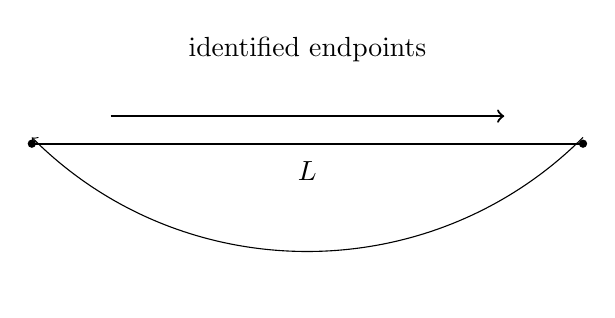
\begin{tikzpicture}[x=1cm,y=1cm]
\draw[thick] (0,0) -- (7,0);
\fill (0,0) circle (1.5pt);
\fill (7,0) circle (1.5pt);
\draw[->,thick] (1.0,0.35) -- (6.0,0.35);
\draw (3.5,-0.35) node{\(L\)};
\draw[->,bend left=45] (7,0.08) to (0,0.08);
\draw (3.5,1.2) node{identified endpoints};
\end{tikzpicture}
\caption{فضاء دوري أحادي البعد يتكون من مطابقة طرفي مسار طوله \(L\).}
\end{figure}

تصل موجة تتحرك إلى اليمين بعد ذلك إلى الطرف المبيَّن، ثم تظهر من جديد عند البداية وتواصل الحركة إلى اليمين. وبالمثل تواصل موجة تتحرك إلى اليسار الحركة إلى اليسار. ولا يوجد طرف مميَّز تنعكس عنده الموجة، لذا لا ينقلب الزخم. يجعل الفضاء الدوري الحجم منتهيًا ويحفظ الزخم، لكن له نتيجة مهمة: الزخوم المسموح بها متقطعة.

يجب أن ينطبق عدد صحيح من الأطوال الموجية على الطول الكلي. وبالنسبة إلى نمط غير ثابت،
\begin{equation}
\lambda_{|N|}=\frac{L}{|N|},
\qquad |N|=1,2,3,\ldots .
\end{equation}
وبالتالي يمكن أن يكون مقدار الطول الموجي \(L\) أو \(L/2\) أو \(L/3\)، وهكذا. أما اختيار مثل \(L/\sqrt{2}\) فلا ينطبق: فبعد دورة كاملة ستعود الموجة بطور غير صحيح ولن تطابق قيمتها الابتدائية.

باستخدام \(p=h/\lambda\)، يكون مقدار الزخم للنمط غير الثابت ذي الرتبة \(|N|\) هو
\begin{equation}
|p_N|=\frac{|N|h}{L}.
\end{equation}
ولإدخال الاتجاهين معًا والنمط الثابت بلا لبس، من الملائم أن يكون دليل النمط ذا إشارة:
\begin{equation}
p_N=\frac{Nh}{L},
\qquad N=0,\pm1,\pm2,\ldots .
\end{equation}
وتصف القيم الموجبة والسالبة لـ \(N\) اتجاهي انتشار متعاكسين. أما النمط \(N=0\) فهو ثابت وزخمه صفري؛ وليس له طول موجي متناهٍ يُدرج في \(h/\lambda\). ولذلك يكون التباعد الأساسي في الزخم هو \(h/L\).

عندما يكون \(L\) عيانيًا، فإن كِلًا من \(h\) و\(1/L\) يجعل هذا التباعد صغيرًا للغاية، بحيث تشكّل القيم المسموح بها مجموعة كثيفة جدًا وتبدو شبه متصلة. ومع ذلك فإن خرزةً مقيَّدة بسلك دائري تمتلك بالضبط هذا الطيف المتقطّع.

\begin{classroomqa}
\lecturetimestamp{00:58:27}
\audiencequestion{هل الكمية المتكمّاة هي الزخم الكلي للموجة، أم الزخم المرتبط بدورة واحدة؟}
\lecturerresponse{تنطبق هذه العبارة على زخم كل كمّ. فلكل كمّ أحد الزخوم المتقطعة المسموح بها. وبالتالي فإن الزخم الكلي لأي مجموعة من الكمّات يكون أيضًا مضاعفًا صحيحًا للوحدة الأساسية \(h/L\).}
\end{classroomqa}

\begin{classroomqa}
\lecturetimestamp{00:59:22}
\audiencequestion{لماذا يجب أن تعود الموجة إلى القيمة نفسها بعد دورة كاملة؟}
\lecturerresponse{الطرفان المتطابقان هما النقطة الفيزيائية نفسها، لذلك يجب أن يكون للحقل القابل للرصد القيمة نفسها عندهما. وأي عدم تطابق سيتطلب قفزة مفاجئة في الحقل عند تلك النقطة. ومثل هذا الانقطاع مكلف من حيث الطاقة والزخم؛ لذا فإن تشكيلات الحقل المسموح بها متصلة ودورية.}
\end{classroomqa}

\begin{classroomqa}
\lecturetimestamp{01:00:09}
\audiencequestion{ماذا يحدث إذا كانت الموجة موضعية في حزمة؟}
\lecturerresponse{الحزمة مجموع فورييه من موجات مستوية، أو بصورة مكافئة من جيوب وجيوب تمام. وفي الفضاء الدوري لا يجوز أن يحتوي هذا المجموع إلا على أنماط الزخم المتقطعة المسموح بها. لذا فإن عبارة التكميم هي عبارة عن مركبات فورييه لكل حزمة مسموح بها.}
\end{classroomqa}

\begin{classroomqa}
\lecturetimestamp{01:01:01}
\audiencequestion{هل توجد مشكلة إذا صار الطول الدوري \(L\) صغيرًا للغاية؟}
\lecturerresponse{كلما تناقص \(L\)، ازداد الزخم الأساسي \(h/L\) كثيرًا. ولا يترتب على ذلك أي عدم اتساق فوري عند الأطوال المجهرية المعتادة، لكن محاولة دفع هذا البناء إلى نطاق طول بلانك يُتوقع أن تتطلب فيزياء جديدة.}
\end{classroomqa}

الآن خذ الصورة الدائرية على نحو حرفي: تتحرك خرزة على سلك دائري نصف قطره \(r\)، ومحيطه \(L=2\pi r\). وزخومها المماسية المسموح بها هي
\begin{equation}
p_N=\frac{Nh}{2\pi r}=\frac{N\hbar}{r}.
\end{equation}
وبالنسبة إلى جسيم غير نسبي في مدار دائري، يكون العزم الزاوي هو \(mvr\). وبما أن \(p=mv\) في ذلك النظام، فهذا يساوي \(rp\). والتعبير \(mvr\) ليس عامًّا نسبيًا، لأن \(p\) عندئذٍ لا يساوي ببساطة \(mv\)، لكن حاصل ضرب الزخم في المسافة العمودية يظل العلاقة الصحيحة. وفي الصورة المتجهية،\footnote{تستعمل المحاضرة أولًا \(L\) للعزم الزاوي، ثم تنتبه إلى تعارضه مع \(L\) للطول الدوري فتغيّر الرموز. وهنا يُستعمل \(J\) على امتداد النص؛ انظر 01:03:40--01:05:21.}
\begin{equation}
\vec J=\vec r\times\vec p,
\end{equation}
وللحركة الدائرية المماسية يكون مقداره \(J=rp\). ومن ثم
\begin{equation}
J_N=rp_N=N\hbar.
\end{equation}
يعتمد تباعد الزخم الخطي على حجم الدائرة، في حين أن وحدة العزم الزاوي هي دائمًا \(\hbar\). وتوجد استثناءات لقاعدة العدد الصحيح عندما تكون الفرميونات داخلة في المسألة؛ وتؤجَّل تلك الاستثناءات.

المهمة التالية هي ربط الحقول بالجسيمات والكمّات على نحو أدق. وهذا يتطلب عودة قصيرة إلى ميكانيكا الكم الخاصة بالمؤثرات والمذبذب التوافقي.

\section{أنماط الموجة والمؤثرات الكمومية}

إن ميكانيكا الكم الآتية لا بد أن تكون مجردة، والمقصود بها المراجعة. والمذبذب التوافقي هو النظام الأساسي لأن الموجة اهتزاز. فعند نقطة ثابتة، يتغير المجال الكهربائي أو المجال المغناطيسي أو أي سعة موجية أخرى دوريًا مع الزمن؛ والقول إن لمركبة ما ترددًا هو في ذاته قول إنها تتذبذب.

لا يلزم أن تكون للموجة العامة طول موجي واحد فقط. إذ يمكن مزج ضوء من عدة ألوان معًا، وبالعكس يمكن لمنشور أن يفصل الضوء المختلط إلى ألوانه المكوِّنة، كما في تحليل Newton للضوء الأبيض. ولكل مركبة طول موجي وتردد وسعة وطاقة وزخم خاص بها. ومن ثم يمكن تحليل الموجة المختلطة إلى كمّات ذات طاقات وزخوم مختلفة. وكل طول موجي يحدد ترددًا، وكل مركبة ذات تردد محدد تسلك سلوك مذبذب. ولهذا كان المذبذب التوافقي، لا أي نظام كمومي اعتباطي، هو اللبنة الأساسية الطبيعية للحقل.

تُمثَّل المرصودات الكمومية بالمؤثرات. ويمكن جمع المؤثرات وضربها، لكن بخلاف الأعداد العادية لا يلزم أن تكون نواتج ضربها مستقلة عن الترتيب. ولتُمثِّل \(A\) و\(B\) خاصيتين لنظام ما، يمكن أن تكون كل منهما قابلة للقياس بمفردها. فعلى سبيل المثال، قد تمثل \(A\) مجالًا كهربائيًا وتمثل \(B\) مجالًا مغناطيسيًا. وإذا كانت القيم المقاسة هي العددين العاديين \(a\) و\(b\)، فإن
\begin{equation}
ab=ba.
\end{equation}
فلا يمكن أن يعتمد حاصل ضربهما العددي على ترتيب الضرب. غير أن المؤثرات المناظرة في ميكانيكا الكم قد تحقق بدلًا من ذلك \(AB-BA\neq0\).

في البداية يبدو هذا غير معقول. فإذا كان قياس المجال الكهربائي يعطي عددًا ما وكان قياس المجال المغناطيسي يعطي عددًا آخر، فلا بد أن يعطي ضرب هذين العددين النتيجة نفسها بأي ترتيب. وحل ذلك هو أنه عندما تعتمد حواصل ضرب المؤثرات على الترتيب، لا يمكن قياس الكميتين معًا في الوقت نفسه. فالتجربة التي تقيس إحداهما تتداخل مع قياس الأخرى. ولا يوجد تناقض، لأن القيمتين العدديتين لا يمكن الحصول عليهما معًا.

عندما يمكن قياس كميتين معًا، تكون قيمتاهما المقاسوَتان عددين عاديين، وهذه الأعداد تتبادل الضرب. ولذلك فإن اختبار إمكان القياس المتزامن هو المبدّل
\begin{equation}
[A,B]=AB-BA.
\end{equation}
ويعني انعدام المبدّل أن المرصودات متوافقة؛ ويعني كون المبدّل غير صفري أن القياسات المناظرة تتداخل. وعكس ترتيب المدخلين يعكس الإشارة:
\begin{equation}
[B,A]=-[A,B].
\end{equation}

بالنسبة إلى جسيم غير نسبي، تتبادل مركبات الموضع الثلاث فيما بينها، وكذلك مركبات الزخم الثلاث:
\begin{align}
[x,y]&=[y,z]=[z,x]=0,\\
[p_x,p_y]&=[p_y,p_z]=[p_z,p_x]=0.
\end{align}
ويمكن تعيين الإحداثيات الثلاثة معًا، ويمكن تعيين مركبات الزخم الثلاث كلها معًا. أما مركبات الموضع والزخم المتناظرة فلا تتبادل الضرب:
\begin{equation}
[x,p_x]=[y,p_y]=[z,p_z]=i\hbar,
\end{equation}
في حين أن المركبات المختلطة مثل \([x,p_y]\) تنعدم. إن قياس إحداثي موضع يُحدث في الجسيم اضطرابًا في الزخم المقترن به. وبصورة مكافئة، فإن حاصل ضرب لا يقينَي الموضع والزخم المناظرين يضبطه \(\hbar\).

\begin{classroomqa}
\lecturetimestamp{01:16:30}
\audiencequestion{عند الانتقال من \(x\) إلى \(y\)، هل ينبغي أن تتغير \(i\) في المبدّل إلى \(j\)؟}
\lecturerresponse{لا. فالرمز \(i\) هو دائمًا الوحدة التخيلية، أي الجذر التربيعي لسالب واحد. وليس هو لا رمزًا لمتجهة وحدة ديكارتية ولا واحدًا من الرموز الكواتيرنيونية \(i,j,k\).}
\end{classroomqa}

\begin{classroomqa}
\lecturetimestamp{01:17:24}
\audiencequestion{هل يعني \(AB-BA\) قياس \(A\) أولًا ثم \(B\)، ثم عكس ترتيب القياس؟}
\lecturerresponse{لا. فالحدّان هما حاصل ضرب مؤثِّرات أو مصفوفات بترتيبين جبريين مختلفين. وهما لا يدلان على تتابع فعلي للقياسات. والارتباط بالقياسات غير المتوافقة هو نتيجة لجبر المؤثِّرات، لا لتعريف الجداء.}
\end{classroomqa}

\begin{classroomqa}
\lecturetimestamp{01:18:32}
\audiencequestion{هل تنطبق مبدِّلات الموضع--الزخم هذه مباشرةً على فوتون؟}
\lecturerresponse{ليس مباشرةً. فهي تنطبق بوضوح على الجسيمات غير النسبية. أما موضع الفوتون فأصعب تعريفًا، ولذلك تتطلب العبارة المناظرة مزيدًا من العناية، ولا نحتاج إليها هنا.}
\end{classroomqa}

\section{المذبذب التوافقي الكمومي}

يوفّر ثقل معلّق بنابض، وموجة صوتية، وموجة ضوئية، أمثلةً كلّها على الحركة الاهتزازية. ولكل مذبذب توافقي مثالي تردد. وبالنسبة إلى النابض، فالدورة الكاملة ليست مجرد الزمن اللازم لعودة الثقل إلى الموضع نفسه؛ بل يجب أن يعود إلى ذلك الموضع وهو يتحرك في الاتجاه نفسه. وعدد الدورات الكاملة في الثانية هو \(f\)، و\(\omega=2\pi f\).

في الوصف الكلاسيكي، يمكن للمذبذب المثالي أن يملك أي طاقة غير سالبة. فدفعة لطيفة تعطي طاقة صغيرة، ودفعة أشد تعطي طاقة أكبر. أما النابض الحقيقي فسينكسر أو ينصهر في النهاية، لكن المثال الرياضي المثالي له مجال متصل من الطاقات الموجبة. ويختلف المذبذب الكمومي: إذ تشكل طاقاته المسموح بها سُلّمًا منفصلًا متساوي التباعد. وإذا اختير مبدأ الطاقة بحيث يُسمّى أدنى مستوى صفرًا،
\begin{equation}
E_n=n\hbar\omega,
\qquad n=0,1,2,\ldots .
\end{equation}
ويمكن تصوير المستويات المتساوية التباعد كما يلي.\footnote{يتبع المخطط التخطيطي لمستويات الطاقة المناقشة على اللوح عند 01:21:20--01:23:56.}

\begin{figure}[t]
\centering
\begin{tikzpicture}[x=1cm,y=0.9cm]
\draw[->] (0,0) -- (0,5.35);
\draw (0,5.5) node[above]{energy};
\foreach \y/\lab in {0.6/{0},1.6/{\hbar\omega},2.6/{2\hbar\omega},3.6/{3\hbar\omega},4.6/{n\hbar\omega}}
{
  \draw[thick] (0.2,\y) -- (2.2,\y);
  \draw (-0.25,\y) node[left]{\(\lab\)};
}
\draw[->,thick] (2.8,0.68) -- (2.8,1.52);
\draw (3.2,1.1) node[right]{\(a_+\)};
\draw[->,thick] (3.7,1.52) -- (3.7,0.68);
\draw (4.1,1.1) node[right]{\(a_-\)};
\end{tikzpicture}
\caption{مستويات المذبذب المتساوية التباعد وفق الاصطلاح \(E_n=n\hbar\omega\).}
\end{figure}

إن التباعد \(\hbar\omega\) هو الطاقة نفسها التي أُسنِدت سابقًا إلى فوتون واحد ذي تردد زاوي \(\omega\). وقد تكون القيمة \(2\hbar\omega\) طاقة كمّ واحد ينتمي إلى مذبذب ذي تردد \(2\omega\)، أو طاقة كمّين في مذبذب ذي تردد \(\omega\). والتفسير الثاني هو المطلوب هنا. ويمكن لمذبذب واحد ذي تردد ثابت أن يحتوي صفرًا أو واحدًا أو اثنين أو ثلاثة أو أكثر من الكمّات، من دون أي طاقات مسموح بها بين الدرجات.

تُوسَم حالة المذبذب بالعدد الصحيح \(n\)، وتُكتب على هيئة كيت \(|n\rangle\). فالحالة \(|0\rangle\) هي الحالة الأرضية، و\(|1\rangle\) فيها كمّ إثارة واحد، و\(|2\rangle\) فيها كمّان، وهكذا. والكيت مجرد ترميز للحالة التي تؤثر فيها المؤثِّرات.

عرّف مؤثِّر رفع \(a_+\) يرفع الحالة مستوى واحدًا، ومؤثِّر خفض \(a_-\) ينزل بها مستوى واحدًا:
\begin{align}
a_+|n\rangle &= \sqrt{n+1}\,|n+1\rangle,\\
a_-|n\rangle &= \sqrt{n}\,|n-1\rangle.
\end{align}
وعوامل الجذر التربيعي العددية جزء من التعريفين. وعلى أدنى حالة،
\begin{equation}
a_-|0\rangle=0,
\end{equation}
لأنه لا توجد حالة تحت الحالة الأرضية.

من المهم هنا التمييز بين الأعداد العادية والمؤثِّرات. فالوسم \(n\) والمعاملات مثل \(\sqrt n\) هي أعداد عادية؛ وهي تتبادل مع كل شيء. أما الرمزان \(a_+\) و\(a_-\) فمؤثِّران، ويجب الحفاظ على ترتيبهما.

اخفض \(|n\rangle\) أولًا، ثم ارفعه من جديد. وتعطي خطوة الخفض
\begin{equation}
a_-|n\rangle=\sqrt n\,|n-1\rangle.
\end{equation}
ويضيف تأثير \(a_+\) على الحالة الناتجة عاملًا آخر هو \(\sqrt n\)، لأن رفع \(|n-1\rangle\) يعيدها إلى \(|n\rangle\):
\begin{align}
a_+a_-|n\rangle
&=a_+\bigl(\sqrt n\,|n-1\rangle\bigr)\\
&=\sqrt n\,\sqrt n\,|n\rangle\\
&=n|n\rangle.
\end{align}
وهكذا يقرأ \(a_+a_-\) رقم المستوى. فافترض مثلًا أن \(|\chi\rangle\) معلوم أنها حالة ذاتية للعدد، لكن وسم مستواها غير معلوم. فإذا كان
\begin{equation}
a_+a_-|\chi\rangle=q|\chi\rangle,
\end{equation}
فإن المعامل العددي العادي \(q\) هو عدد الكمّات في تلك الحالة. ولذلك يكون هذا الجداء هو مؤثِّر العدد،
\begin{equation}
\hat n=a_+a_-,
\end{equation}
وبحسب اصطلاح الطاقة المختار يكون الهاملتوني
\begin{equation}
H=\hbar\omega\,a_+a_-.
\end{equation}
وبالفعل فإن تأثيره على أي مستوى يعطي \(H|n\rangle=n\hbar\omega|n\rangle\).

والآن اعكس الترتيب. فالرفع أولًا يعطي \(\sqrt{n+1}|n+1\rangle\). ثم يعيد الخفض إلى \(|n\rangle\) ويعطي عاملًا ثانيًا \(\sqrt{n+1}\):
\begin{align}
a_-a_+|n\rangle
&=a_-\bigl(\sqrt{n+1}\,|n+1\rangle\bigr)\\
&=\sqrt{n+1}\,\sqrt{n+1}\,|n\rangle\\
&=(n+1)|n\rangle.
\end{align}
ويختلف الترتيبان بمقدار واحد على كل حالة، لذلك
\begin{equation}
[a_-,a_+]=a_-a_+-a_+a_-=1.
\end{equation}

للمذبذب كذلك سعة وطور. ويحدد طوره موضعه في دورته؛ وبصورة ملموسة، يمكن تثبيته بالزمن الذي يمر فيه المذبذب عبر الأصل في اتجاه مختار. وتأخير ذلك العبور يغيّر الطور من دون أن يغيّر التردد. وتجمع مؤثِّرات السلم المتغيرات الكمومية المرتبطة بالسعة والطور. وجبرها كمومي في جوهره، لكن فعلها بسيط: يضيف \(a_+\) كمًّا واحدًا من طاقة المذبذب ويزيل \(a_-\) كمًّا واحدًا. وبالنسبة إلى نمط كهرومغناطيسي، تكون تلك الكمّات فوتونات، ولذلك يسمّى المؤثِّران مؤثِّري الإنشاء والإفناء.

\begin{classroomqa}
\lecturetimestamp{01:37:34}
\audiencequestion{هل يقابل مؤثِّرا الرفع والخفض قياسًا فيزيائيًا؟}
\lecturerresponse{عدد الفوتونات قابل للقياس. أما المؤثِّران \(a_+\) و\(a_-\) فليسا مرصودين قابلين للقياس، كلٌّ على حدة، وذلك لأسباب تقنية إضافية. ويُظهر مبدّلهما أن الاثنين لا يتبادلان، لكن هذه الحقيقة وحدها ليست الحجة على أن أيًّا منهما، منفردًا، غير قابل للرصد.}
\end{classroomqa}

تعطي مجموعة من النوابض ذات الترددات الطبيعية المختلفة مذبذبات مستقلة كثيرة. وكذلك تفعل الأنماط الكهرومغناطيسية في تجويف: إذ يمكن إثارة طول موجي واحد من غير أن يُلزِم ذلك الأطوال الأخرى بأن تكون لها الإثارة نفسها. وكموميًا، تضيف مؤثِّرات الإنشاء والإفناء كمّات ذات تردد ثابت وتزيلها في كل مذبذب مستقل. وهذه اللغة مركزية لأن الجسيمات ستُعرَّف على أنها تلك الكمّات بالضبط.

\section{حقل بوصفه مجموعة من المذبذبات}

لنعد إلى فضاء دوري أحادي البعد طوله الكلي \(L\). ولأنماطه غير الثابتة مقادير أطوال موجية
\begin{equation}
\lambda_N=\frac{L}{N},
\qquad N=1,2,3,\ldots ,
\end{equation}
وترددات زاوية غير سالبة مناظرة \(\omega_N\). ولأجل المقارنة مع طيف الزخم السابق، من المفيد إعادة تسمية عدده الصحيح ذي الإشارة بـ \(M\):
\begin{equation}
p_M=\frac{Mh}{L},
\qquad M=0,\pm1,\pm2,\ldots .
\end{equation}
وتسجل إشارة \(M\) اتجاه الانتشار.
\editorialnote{عند 01:42:08--01:42:24، يُصحَّح دليل نمط التردد من مجال ذي إشارة إلى مجال يبدأ من الصفر صعودًا. ويُستعمل الرمز \(M\) هنا فقط للإبقاء على ترميز الزخم ذي الإشارة منفصلًا عن وسم نمط التردد غير السالب \(N\)؛ ولا يُدخل إشغالات مستقلة لكل من \(+M\) و\(-M\). وتبدأ قائمة المذبذبات غير الثابتة عند \(N=1\).}

يتصرف كل تردد مسموح به كمذبذب توافقي. ويمكن إضافة الطاقة على نحو مستقل إلى تردد واحد ثم إلى آخر. ويُرجأ المثال الأول المفصل لحقل كمومي إلى المحاضرة التالية، لكن ترميز الحالة واضح بالفعل. وبترتيب الأنماط غير الثابتة من أطول طول موجي فصاعدًا، اكتب
\begin{equation}
|n_1,n_2,n_3,\ldots\rangle,
\end{equation}
حيث إن \(n_N=0,1,2,\ldots\) هو عدد الكمّات في المذبذب ذي التردد \(\omega_N\). ويدل المدخل الأول على عدد الكمّات التي تشغل نمط أطول طول موجي، ويدل الثاني على عدد الكمّات التي تشغل النمط التالي، وهكذا إلى غير نهاية.

تجعل توافقيات الوتر هذا البناء ملموسًا. ويُعرض تخطيطيًا التدرج من النمط الأساسي إلى التوافقيين التاليين.\footnote{يتبع هذا الشكل التخطيطي مناقشة توافقيات الوتر عند 01:45:20--01:47:46.}

\begin{figure}[t]
\centering
\resizebox{\linewidth}{!}{%
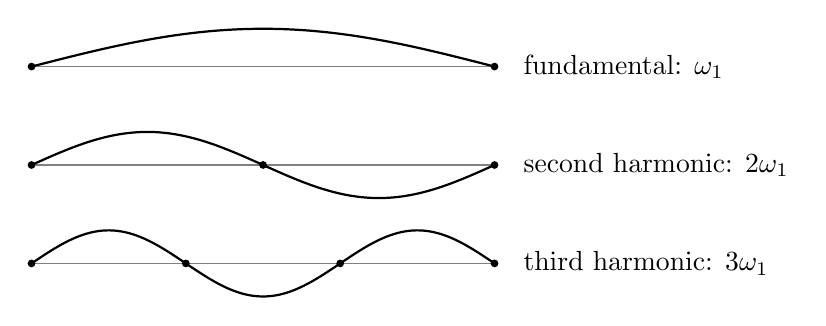
\begin{tikzpicture}[x=0.98cm,y=1cm]
\draw[gray] (0,2.5) -- (6,2.5);
\draw[thick] plot[domain=0:6,samples=120] (\x,{2.5+0.48*sin(30*\x)});
\fill (0,2.5) circle (1.4pt);
\fill (6,2.5) circle (1.4pt);
\node[right] at (6.25,2.5) {fundamental: \(\omega_1\)};

\draw[gray] (0,1.25) -- (6,1.25);
\draw[thick] plot[domain=0:6,samples=120] (\x,{1.25+0.42*sin(60*\x)});
\fill (0,1.25) circle (1.4pt);
\fill (3,1.25) circle (1.4pt);
\fill (6,1.25) circle (1.4pt);
\node[right] at (6.25,1.25) {second harmonic: \(2\omega_1\)};

\draw[gray] (0,0) -- (6,0);
\draw[thick] plot[domain=0:6,samples=120] (\x,{0.42*sin(90*\x)});
\fill (0,0) circle (1.4pt);
\fill (2,0) circle (1.4pt);
\fill (4,0) circle (1.4pt);
\fill (6,0) circle (1.4pt);
\node[right] at (6.25,0) {third harmonic: \(3\omega_1\)};
\end{tikzpicture}%
}
\caption{النمط الأساسي للوتر وتوافقيه الثاني والثالث، مع عدم وجود عقد داخلية، ثم عقدة داخلية واحدة، ثم عقدتين داخليتين.}
\end{figure}

يتحرك النمط الأساسي على هيئة قوس عريض واحد، وليس له أي عقدة داخلية. وهو مذبذب واحد، وقد يكون عدد كمّاته \(n_1=0,1,2,\ldots\)؛ وتكلفة كل إثارة هي \(\hbar\omega_1\). وللتوافقي الثاني عقدة داخلية واحدة وتردده ضعف تردد النمط الأساسي. فإذا كان النمط الأساسي يصدر نغمة دو الوسطى، فإن هذا النمط يصدر نغمة دو على بعد أوكتاف أعلى. وله عدد إشغال مستقل \(n_2\)، وتكلفة كل كمّ من كمّاته هي \(\hbar\omega_2=2\hbar\omega_1\). أما التوافقي الثالث فله عقدتان داخليتان وثلاثة أمثال تردد النمط الأساسي. وله عدد إشغال مستقل خاص به \(n_3\)، ويمكن مرة أخرى أن يكون أي عدد صحيح غير سالب.

نمطًا بنمط، وفي اصطلاح الطاقة المستخدم أعلاه، تكون الطاقة مساوية لعدد الإشغال مضروبًا في طاقة الكم. وجمع هذه المساهمات يعطي
\begin{equation}
E=\sum_{N=1}^{\infty} n_N\hbar\omega_N.
\end{equation}
\editorialnote{هذا المجموع المعروض هو الجمع الجبري لطاقات الأنماط المذكورة كلٌّ على حدة عند 01:44:02--01:47:46.}

يجب تكرار رياضيات المذبذب التوافقي نفسها لكل نمط حقلي، مع مؤثِّر إنشاء واحد ومؤثِّر إفناء واحد لكل مذبذب مستقل. وفي هذا التصور الابتدائي الأول، يكون الحقل الكمومي هو تلك المجموعة الكاملة من المذبذبات وجبر الإنشاء--الإفناء الخاص بها.

هذه اللغة مكيَّفة مع تشتت الجسيمات. تدخل إلى التجربة كمّات ذات طاقة وزخم محددين، وتغادرها كمّات ذات طاقات وزخوم أخرى. تُزال الجسيمات الابتدائية بمؤثرات الإفناء؛ وتُدرَج الجسيمات الخارجة في الحالة النهائية بمؤثرات الخلق الخاصة بالأنماط المناسبة.

\begin{classroomqa}
\lecturetimestamp{01:49:38}
\audiencequestion{هل يُستعمل العدد الصحيح نفسه لوسم نمط المذبذب ولعدِّ عدد الكمّات فيه؟}
\lecturerresponse{هناك عددان صحيحان متميزان. فوسم النمط \(N\) يحدد النمط المكاني؛ وفي مثال الوتر، يحدد عددُ عُقَده التردد \(\omega_N\). أمّا عدد الإشغال \(n_N\) فيبيّن كم عددَ الكمّات التي لها ذلك التردد.}
\end{classroomqa}